% ---------------------------------------------------------------------------
% main.tex — deck template (theme preview only)
%
% This file holds no project content on purpose: it exists to show the layout
% and the colour scheme. Slides are built by copying the frame skeletons below.
%
% Build:  latexmk -pdf main.tex      (or: pdflatex main.tex, twice)
% Theme:  theme.tex — palette, chrome, boxes, code style. Nothing visual here.
% ---------------------------------------------------------------------------

\documentclass[aspectratio=169, 11pt]{beamer}

% ---------------------------------------------------------------------------
% theme.tex — layout and colour scheme for the project slide deck
%
% Deliberately minimal: a coloured title rule, a quiet footer, and flat
% callouts. Everything visual lives in this file, so the palette or the chrome
% can be changed without touching a single slide.
%
% Load order: \input this after \documentclass{beamer}. It loads what it needs.
% ---------------------------------------------------------------------------

\usepackage[T1]{fontenc}
\usepackage{lmodern}
\usepackage{tikz}
\usetikzlibrary{arrows.meta, positioning, calc, fit, backgrounds, shapes.geometric}
\usepackage[most]{tcolorbox}
\usepackage{booktabs}
\usepackage{listings}
\usepackage{xcolor}
\usepackage{amsmath,amssymb}

% ---------------------------------------------------------------------------
% 1. Palette — five colours, and three neutrals
%
% Re-skin the whole deck by changing these values. Nothing else in this file
% or in main.tex hard-codes a colour.
% ---------------------------------------------------------------------------

\definecolor{rtmPrimary}{HTML}{12314F}   % deep navy   — titles, rules, structure
\definecolor{rtmAccent}{HTML}{0E9AA7}    % teal        — emphasis, arrows, bullets
\definecolor{rtmAlert}{HTML}{E8833A}     % amber       — warnings, "before"
\definecolor{rtmGood}{HTML}{2E9E5B}      % green       — results, "after"
\definecolor{rtmInk}{HTML}{1F2933}       % body text
\definecolor{rtmMuted}{HTML}{6B7A8F}     % captions, footer, secondary
\definecolor{rtmLine}{HTML}{D5DEE7}      % hairlines, table rules
\definecolor{rtmSurface}{HTML}{EDF2F7}   % box fill, code background

% ---------------------------------------------------------------------------
% 2. Beamer colours and fonts
% ---------------------------------------------------------------------------

\setbeamercolor{normal text}{fg=rtmInk, bg=white}
\setbeamercolor{structure}{fg=rtmPrimary}
\setbeamercolor{frametitle}{fg=rtmPrimary, bg=white}
\setbeamercolor{title}{fg=rtmPrimary}
\setbeamercolor{subtitle}{fg=rtmMuted}
\setbeamercolor{author}{fg=rtmInk}
\setbeamercolor{date}{fg=rtmMuted}
\setbeamercolor{itemize item}{fg=rtmAccent}
\setbeamercolor{itemize subitem}{fg=rtmMuted}
\setbeamercolor{enumerate item}{fg=rtmAccent}
\setbeamercolor{alerted text}{fg=rtmAccent}
\setbeamercolor{footline}{fg=rtmMuted}
\setbeamercolor{block title}{fg=white, bg=rtmPrimary}
\setbeamercolor{block body}{fg=rtmInk, bg=rtmSurface}
\setbeamercolor{block title alerted}{fg=white, bg=rtmAlert}
\setbeamercolor{block body alerted}{fg=rtmInk, bg=rtmSurface}
\setbeamercolor{block title example}{fg=white, bg=rtmGood}
\setbeamercolor{block body example}{fg=rtmInk, bg=rtmSurface}

\setbeamerfont{frametitle}{size=\large, series=\bfseries}
\setbeamerfont{title}{size=\LARGE, series=\bfseries}
\setbeamerfont{subtitle}{size=\large}
\setbeamerfont{author}{size=\small}
\setbeamerfont{footline}{size=\tiny}
\setbeamerfont{caption}{size=\scriptsize}

% ---------------------------------------------------------------------------
% 3. Frame chrome
%
% A short teal rule above the frame title, the title in navy, and a hairline
% under it. The footer carries the short title on the left and the page number
% on the right. No navigation symbols, no colour band across the slide.
% ---------------------------------------------------------------------------

\useinnertheme{default}
\useoutertheme{default}
\setbeamertemplate{navigation symbols}{}
\setbeamersize{text margin left=8mm, text margin right=8mm}

\setbeamertemplate{frametitle}{%
  \vskip3mm%
  {\color{rtmAccent}\hrule height 1.4pt width 18mm}%
  \vskip2mm%
  {\usebeamerfont{frametitle}\usebeamercolor[fg]{frametitle}%
   \insertframetitle\par}%
  \vskip1.6mm%
  {\color{rtmLine}\hrule height 0.4pt}%
  \vskip1.5mm%
}

\setbeamertemplate{footline}{%
  \hbox to\paperwidth{%
    \hskip8mm%
    {\usebeamerfont{footline}\usebeamercolor[fg]{footline}%
      \insertshortauthor\hskip1em\textbar\hskip1em\insertshorttitle}%
    \hfill%
    {\usebeamerfont{footline}\usebeamercolor[fg]{footline}%
      \insertframenumber\,/\,\inserttotalframenumber}%
    \hskip8mm%
  }%
  \vskip2.2mm%
}

% ---------------------------------------------------------------------------
% 4. Title page
%
% A navy band across the top third, with the teal rule under it. The lower
% part of the slide stays white, which is where a university logo would go.
% ---------------------------------------------------------------------------

\setbeamertemplate{title page}{%
  \begin{tikzpicture}[remember picture, overlay]
    \fill[rtmPrimary]
      (current page.north west) rectangle ([yshift=-0.47\paperheight]current page.north east);
    \fill[rtmAccent]
      ([yshift=-0.47\paperheight]current page.north west)
      rectangle ([yshift=-0.478\paperheight]current page.north east);
    \node[anchor=north west, inner sep=0pt, text width=0.84\paperwidth]
      at ([xshift=8mm, yshift=-12mm]current page.north west) {%
        {\color{rtmAccent}\footnotesize\bfseries\insertinstitute}\par
        \vskip3mm
        {\color{white}\LARGE\bfseries\inserttitle}\par
        \vskip2.5mm
        {\color{rtmAccent!65!white}\large\insertsubtitle}\par
      };
    \node[anchor=south west, inner sep=0pt, text width=0.84\paperwidth]
      at ([xshift=8mm, yshift=8mm]current page.south west) {%
        {\color{rtmInk}\small\insertauthor}\par
        \vskip2mm
        {\color{rtmMuted}\small\insertdate}\par
      };
  \end{tikzpicture}%
}

% ---------------------------------------------------------------------------
% 5. Section pages
%
% A plain slide with the section number in teal above the section name.
% ---------------------------------------------------------------------------

\AtBeginSection[]{%
  \begin{frame}[plain]
    \vfill
    {\color{rtmAccent}\hrule height 1.4pt width 18mm}\par
    \vskip3mm
    {\color{rtmAccent}\small\bfseries PART \insertsectionnumber\par}
    \vskip1.5mm
    {\color{rtmPrimary}\LARGE\bfseries\insertsectionhead\par}
    \vfill
  \end{frame}%
}

% ---------------------------------------------------------------------------
% 6. Boxes — one left accent bar on a neutral fill, nothing else
% ---------------------------------------------------------------------------

\newtcolorbox{highlight}[1][]{%
  enhanced, breakable,
  colback=rtmSurface, colframe=rtmAccent,
  boxrule=0pt, leftrule=2.4pt, arc=0pt, outer arc=0pt,
  left=2.5mm, right=2mm, top=1.6mm, bottom=1.6mm,
  fontupper=\small, #1}

\newtcolorbox{tech}[1][]{%
  enhanced, breakable,
  colback=rtmSurface, colframe=rtmPrimary,
  boxrule=0pt, leftrule=2.4pt, arc=0pt, outer arc=0pt,
  left=2.5mm, right=2mm, top=1.6mm, bottom=1.6mm,
  fontupper=\small, #1}

\newtcolorbox{warn}[1][]{%
  enhanced, breakable,
  colback=rtmSurface, colframe=rtmAlert,
  boxrule=0pt, leftrule=2.4pt, arc=0pt, outer arc=0pt,
  left=2.5mm, right=2mm, top=1.6mm, bottom=1.6mm,
  fontupper=\small, #1}

% ---------------------------------------------------------------------------
% 7. Tables, code, diagrams, shorthands
% ---------------------------------------------------------------------------

\setbeamertemplate{caption}[numbered]
\newcommand{\rtmtablehead}[1]{{\color{rtmPrimary}\bfseries #1}}
\renewcommand{\arraystretch}{1.15}

\lstdefinestyle{rtmc}{%
  language=C,
  basicstyle=\ttfamily\scriptsize,
  keywordstyle=\color{rtmPrimary}\bfseries,
  commentstyle=\color{rtmMuted}\itshape,
  stringstyle=\color{rtmAccent},
  numberstyle=\ttfamily\tiny\color{rtmMuted},
  backgroundcolor=\color{rtmSurface},
  frame=none, framesep=1.5mm, xleftmargin=2mm,
  aboveskip=1.5mm, belowskip=1.5mm,
  showstringspaces=false, breaklines=true,
  columns=fullflexible, keepspaces=true, upquote=true,
}
\lstset{style=rtmc}

\tikzset{
  node distance=6mm and 9mm,
  block/.style={rectangle, rounded corners=1.2pt, draw=rtmPrimary, line width=0.5pt,
                fill=white, text=rtmInk, align=center,
                inner xsep=2.4mm, inner ysep=1.6mm, font=\scriptsize},
  accent block/.style={block, draw=rtmAccent, fill=rtmAccent!8},
  muted block/.style={block, draw=rtmMuted, fill=rtmSurface, text=rtmMuted},
  flow/.style={-{Latex[length=1.6mm]}, draw=rtmAccent, line width=0.6pt},
  flow dashed/.style={flow, dashed},
  edge label/.style={font=\tiny, text=rtmMuted, inner sep=1pt},
}

% \concept{…} — teal bold inline emphasis (not \tag: beamer owns that name)
\newcommand{\concept}[2][rtmAccent]{{\color{#1}\bfseries #2}}

% \num{1.25} — a number the eye should catch
\newcommand{\num}[1]{\textcolor{rtmAccent}{\bfseries #1}}

% \key{…} — a short label in a navy pill, for a slide's takeaway
\newcommand{\key}[1]{%
  \tikz[baseline=(k.base)]\node[fill=rtmPrimary, text=white, rounded corners=1pt,
    inner xsep=2mm, inner ysep=0.8mm, font=\scriptsize\bfseries] (k) {#1};}


% ---------------------------------------------------------------------------
% Deck metadata — the title block, written once
% ---------------------------------------------------------------------------

\title[RT-MOMS]{Real-Time Multi-Core Sorting and Median Filter Service}
\subtitle{26ELC331 — Real-Time Operating Systems}
\author{%
  Anmol Govindarajapuram Krishnan — CB.EN.U4EEE23103\\
  Mauli Rajguru — CB.EN.U4EEE23120\\
  Sanjay TS — CB.EN.U4EEE23136%
}
\institute{Amrita Vishwa Vidyapeetham}
\date{\today}

\newcommand{\shortauth}{Anmol G. K., Mauli R., Sanjay TS}
\author[\shortauth]{%
  Anmol Govindarajapuram Krishnan — CB.EN.U4EEE23103\\
  Mauli Rajguru — CB.EN.U4EEE23120\\
  Sanjay TS — CB.EN.U4EEE23136%
}

\begin{document}

% ===========================================================================
% 1. Title slide
% ===========================================================================

\begin{frame}[plain]
  \titlepage
\end{frame}

% ===========================================================================
% 2. Layout preview — run this once, then delete it
%
% Every element the deck can use, on one slide, so the look can be judged at a
% glance. Nothing here is content.
% ===========================================================================

\begin{frame}{Layout preview — text, table, code}
  \begin{columns}[t, onlytextwidth]
    % ---- left column: headings, bullets, emphasis ----
    \begin{column}{0.50\textwidth}
      {\color{rtmMuted}\scriptsize\bfseries SECTION HEADING}\par
      \vskip1mm
      \begin{itemize}
        \item First-level bullet with \concept{inline emphasis}
        \item A second bullet, and a \num{42.7\%} figure in accent colour
        \begin{itemize}
          \item A sub-item, quieter than its parent
        \end{itemize}
        \item Third bullet, closing the list
      \end{itemize}
      \vskip2mm
      {\color{rtmMuted}\scriptsize\bfseries EMPHASIS}\par
      \vskip1mm
      Body text in the normal ink colour, sized for projection, and
      \alert{alerted text} for something that must not be missed.
    \end{column}

    % ---- right column: table and callout ----
    \begin{column}{0.46\textwidth}
      \begin{table}
        \centering
        \begin{tabular}{@{}lr@{}}
          \toprule
          \rtmtablehead{Quantity} & \rtmtablehead{Value} \\
          \midrule
          First row   & 1 \\
          Second row  & 2 \\
          Third row   & \num{3} \\
          \bottomrule
        \end{tabular}
      \end{table}
      \vskip1mm
      \begin{highlight}
        \textbf{Highlight box} — teal rule, for a point worth remembering.
      \end{highlight}
    \end{column}
  \end{columns}
\end{frame}

% ---------------------------------------------------------------------------
\begin{frame}[fragile]{Layout preview — boxes, code, diagram}
  \begin{columns}[t, onlytextwidth]
    \begin{column}{0.48\textwidth}
      \begin{tech}
        \textbf{Technical box} — navy rule, for an implementation note.
      \end{tech}
      \vskip2mm
      \begin{warn}
        \textbf{Warning box} — amber rule, for a caveat or a risk.
      \end{warn}
      \vskip3mm
      \key{Pill: one line, the slide's takeaway}
    \end{column}

    \begin{column}{0.50\textwidth}
\begin{lstlisting}[numbers=left]
/* Code block --- monospaced, */
int example(int n)          /* line numbers optional */
{
    return n * n;
}
\end{lstlisting}
      \vskip1mm
      \begin{center}
      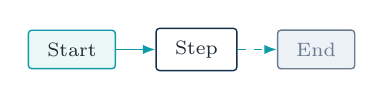
\begin{tikzpicture}[node distance=6mm and 5mm]
        \node[accent block] (a) {Start};
        \node[block, right=of a] (b) {Step};
        \node[muted block, right=of b] (c) {End};
        \draw[flow] (a) -- (b);
        \draw[flow dashed] (b) -- (c);
      \end{tikzpicture}
      \end{center}
    \end{column}
  \end{columns}
\end{frame}

% ===========================================================================
% 3. Closing slide
% ===========================================================================

\begin{frame}[plain]
  
\begin{tikzpicture}[remember picture, overlay]
    \fill[rtmPrimary]
      (current page.north west) rectangle ([yshift=-0.40\paperheight]current page.north east);
    \fill[rtmAccent]
      ([yshift=-0.40\paperheight]current page.north west)
      rectangle ([yshift=-0.408\paperheight]current page.north east);
    \node[anchor=north west, inner sep=0pt, text width=0.84\paperwidth]
      at ([xshift=8mm, yshift=-12mm]current page.north west) {%
        {\color{rtmAccent}\footnotesize\bfseries THANK YOU}\par
        \vskip4mm
        {\color{white}\Large\bfseries Real-Time Multi-Core Sorting and Median Filter Service}\par
      };
    \node[anchor=south west, inner sep=0pt, text width=0.84\paperwidth]
      at ([xshift=8mm, yshift=10mm]current page.south west) {%
        {\color{rtmInk}\small Anmol Govindarajapuram Krishnan — CB.EN.U4EEE23103}\par
        {\color{rtmInk}\small Mauli Rajguru — CB.EN.U4EEE23120}\par
        {\color{rtmInk}\small Sanjay TS — CB.EN.U4EEE23136}\par
        \vskip2mm
        {\color{rtmMuted}\scriptsize 26ELC331 — Real-Time Operating Systems}
      };
  \end{tikzpicture}%
\end{frame}

\end{document}
